\documentclass[a4paper,14pt]{book}
%\documentclass[a4paper]{book}
% \linespread{2.}
%\documentclass[12pt]{article}
%\documentclass[12pt]{cmmp}

%%\usepackage{psfig}
%\usepackage{harvard}
\usepackage{epsfig}
%%\usepackage{amsmath}
\usepackage{amsfonts}
%%\usepackage{amssymb}
%%\usepackage{graphicx}
%%
%%\usepackage{txfonts}
%%%\usepackage{mathrsfs}
%
%\usepackage{feynmf}     %<------------ Obbligatorio
\unitlength=1mm         %<------------ Obbligatorio
%
\newcommand{\braket}[1]{\langle {#1} \rangle }
\newcommand{\ket}[1]{|{#1} \rangle }
\newcommand{\bra}[1]{\langle {#1}|}
\usepackage{latexsym}
\usepackage{amssymb}
\usepackage{amsmath}
\usepackage[varg]{txfonts}
\usepackage{mathrsfs}
\usepackage{upgreek}
%\usepackage [latin1]{inputenc}
\usepackage{verbatim}
\usepackage{array}
\usepackage{color}
%\pagestyle{plain}
\usepackage{graphicx}
\DeclareMathAlphabet{\mathpzc}{OT1}{pzc}{m}{it}



\begin{document}
 \setcounter{chapter}{3}



\chapter{Beyond mean field: particle-vibration coupling}

Inserting the expression given in Eq.(\ref{eqn:29}) in the expression of the empirical potential given in Eq.(\ref{eqn:6}) and expanding to lowest order in $\alpha_{LM}$ (note that $\beta_L^2 \ll \beta_L$, cf. Eq.(\ref{eqn:25})) one obtains

\begin{equation}
H = H_M + H_{coupl} + H_{coll} ,
\label{eqn:30}
\end{equation}

\noindent where

\begin{equation}
H_{coupl} = -\kappa \hat{\alpha} \hat{F} ,
\label{eqn:31}
\end{equation}

\noindent with

\begin{equation}
\hat{F} = \sum_{\nu_1 \nu_2} \langle \nu_1|F|\nu_2 \rangle a_{\nu_1}^{\dagger} a_{\nu_2} ,
\label{eqn:32}
\end{equation}

\noindent and

\begin{equation}
F = - \frac{1}{\kappa} R_0 \frac{\partial U(r)}{\partial r} Y_{LM}^* (\hat{r}) .
\label{eqn:33}
\end{equation}

\noindent The Hamiltonian $H_{coupl}$ thus couples the motion of a single-nucleons with the collective vibrations of the surface, with a matrix element (cf. Fig.\ref{fig:4.1})

\begin{equation}
\langle n_{\alpha} = 1, \nu' |H_{coupl}|\nu \rangle = \Lambda_{\alpha} \langle \nu' |F|\nu \rangle = \langle n_{\alpha}=1, \nu\nu'|H_{coupl}|0 \rangle ,
\label{eqn:34}
\end{equation}

\noindent where

\begin{equation}
\Lambda_{\alpha} = -\kappa \sqrt{\frac{\hbar\omega_{\alpha}}{2C_{\alpha}}} \sim -\frac{\kappa \beta_{\alpha}}{\sqrt{2L_{\alpha}+1}} ,
\label{eqn:35}
\end{equation}

\noindent is the particle-vibration coupling strength. Because $\beta_L^2 \ll \beta_L$, one can usually treat the particle-vibration coupling in the weak coupling situation. Consequently $H_{coul}$, can be treated in perturbation theory. To second order one finds (cf. App. F)

\begin{eqnarray}
\nonumber
( -\frac{\hbar^2}{2m} \nabla_r^2 &+& U_H(r)) \varphi_{\gamma}(r) + \int {\rm d}^3 r' U_x(\vec{r},\vec{r'})\varphi_j(\vec{r'}) \\
\nonumber
&+& (\Delta E +iW_j)\varphi_j(\vec{r}) \\
&\approx& \left( -\frac{\hbar^2}{2m_k} \nabla_r^2 + U_H^"(r) + \Delta E_j + iW_j \right) \varphi_j(\vec{r}) \\
\nonumber
&=& \varepsilon_j\varphi_j(\vec{r}), \;\;\;\;\;\; \left( U_H^" = \frac{m}{m_k} U \right) \\
\label{eqn:36}
\end{eqnarray}

\noindent where (cf. Fig.\ref{fig:4.2})

\begin{equation}
\Delta E_j^{(\omega)} = {\rm Re} \sum_j(\omega) = \lim_{\Delta \rightarrow 0} \sum_{\alpha'} \frac{V_{\nu ,\alpha'}^2 (\omega-E_{\alpha'})}{(\omega -E_{\alpha'})^2 + (\frac{\Delta}{2})^2}
\label{eqn:37a}
\end{equation}

\noindent and

\begin{equation}
W_j^{(\omega)} = {\rm Im} \sum_j(\omega) = \lim_{\Delta \rightarrow 0} \sum_{\alpha'} \frac{V_{\nu ,\alpha'}^2}{(\omega -E_{\alpha'})^2 + (\frac{\Delta}{2})^2}
\label{eqn:37b}
\end{equation}

\noindent are the real and imaginary contributions to the self-energy calculated in second order perturbation theory \footnote{Given a Hamiltonian $H_{coupl}$, the contribution to the energy in second order perturbation theory is

{\protect
\begin{equation}
\Sigma_{\nu}(\omega) = \sum_{\alpha'} \frac{V_{\nu ,\alpha'}^2}{\omega - E_{\alpha'}} ,
\label{eqn:37c}
\end{equation}
}

\noindent where $|\alpha' \rangle \equiv |n_{\alpha}=1,\nu' \rangle$ are the intermediate states which can couple to the initial single-particle state $\nu$. Note that the expression above is not well defined, in that the energy denominator may vanish. As a rule, textbooks in quantum mechanics deal with such a situation by stating that accidental degeneracies are to be eliminated by diagonalization. Now, this is not a real solution of the problem, because it does not contemplate the case where there are many intermediate state with $E_{\alpha'} \approx \omega$, in other words, where the particle can decay into a more complicated state, starting in the single-particle level $\nu$ of energy $\omega$, without changing its energy (real process). This is a typical dissipative (diffusion) process, and has to be solved by direct diagonalization (cf. Fig.\ref{fig:4.5}). Another way around, is to extend the function $\sum_{\nu}(\omega)$ into the complex plane $(E_{\alpha'} \rightarrow E_{\alpha'} + \frac{i\Delta}{2})$ thus {\it regularizing the divergence}, determining the finite contributions and then taking the limit for $\Delta \rightarrow 0$ (Eqs.(\ref{eqn:37a}) and (\ref{eqn:37b})). The resulting complex potential ({\it optical potential} from the {\it complex dielectric function} of optics), parametrizes in simple terms the shift of the centroid of the single-particle state and its finite lifetime.}.

Furthermore,

\begin{equation}
\nonumber
E_{\alpha'} = \varepsilon_{\nu'} + \hbar \omega_{\alpha},
\end{equation}

\noindent and

\begin{equation}
\nonumber
V_{\nu ,\alpha'} = \langle n_{\alpha}=1,\nu'|H_{coupl}|\nu \rangle .
\end{equation}

\begin{figure}[h!]
\centerline {
{\includegraphics*[width=\textwidth]{figs_C4S/fig_4_1}}
}
\caption{Schematic representation of the process by which a nucleon excites the vibrations of the surface.}
\label{fig:4.1}
\end{figure}

\begin{figure}[h!]
\centerline {
{\includegraphics*[width=\textwidth]{figs_C4S/fig_4_2}}
}
\caption{Self-energy graph for a single-particle}
\label{fig:4.2}
\end{figure}

For most purposes $\Delta E$ can be treated in terms of an effective mass (cf. App. C, H and Z)

\begin{equation}
m_{\omega} = m(1+\lambda),
\label{eqn:38}
\end{equation}

\noindent where

\begin{equation}
\lambda= - \frac{\partial \Delta E}{\partial \omega},
\label{eqn:39}
\end{equation}

\noindent is the {\it mass enhancement factor}, while

\begin{equation}
\nonumber
Z_{\omega}=m/m_{\omega},
\end{equation}

\noindent is the spectroscopic factor (discontinuity of the Fermi energy).

Consequently, Eq.(\ref{eqn:36}) can be rewritten as

\begin{equation}
\left( - \frac{\hbar^2}{2m^*} \nabla_r^2 + U_H' + i W(\omega) \right) \varphi_j(\vec{r}) = \varepsilon_j \varphi_j(\vec{r}),
\label{eqn:40a}
\end{equation}

\noindent with

\begin{equation}
m^* = \frac{m_k m_{\omega}}{m} .
\label{eqn:40b}
\end{equation}

\noindent and $U'_H = (m/m^*) U$. Because $\lambda \approx 0.5$ (i.e. the dressed single-particle $m_{\omega}$ is heavier than the bare nucleon, as it has to carry a phonon along), $m^* \approx 1$ and $Z_{\omega} \approx 0.7$. Furthermore, due to the fact that $\hbar \omega_{\alpha} \approx 2-2.5 MeV$, {\it the range} of single-particle energy $E=\varepsilon-\varepsilon_F$ over which the particle-vibration coupling process displayed in Fig.\ref{fig:4.2} effective is $\approx \pm 2\hbar \omega_{\alpha} \approx 4-5$ around the Fermi energy (cf. Figs.\ref{fig:4.3} and \ref{fig:4.4})

\begin{figure}[h!]
\centerline {
{\includegraphics*[width=\textwidth]{figs_C4S/fig_4_3}}
}
\caption{Schematic representation of the $\omega$-mass as a function of the single-particle energy.}
\label{fig:4.3}
\end{figure}

\begin{figure}[h!]
\centerline {
{\includegraphics*[width=\textwidth]{figs_C4S/fig_4_4}}
}
\caption{Schematic representation of the behaviour of $m_{\omega}/m$, $Z_{\omega}=(m_{\omega}/m)^{-1}$ and $\Gamma$ as a function of $E = \varepsilon - \varepsilon_F$.}
\label{fig:4.4}
\end{figure}


To be noted that $\Delta E_j$ (Eq.(\ref{eqn:37a})) indicates the shift in energy of the energy centroid of the "dressed" single-particle state due to the coupling to the intermediate (more complex states) $\alpha' \equiv (\nu',\alpha)$, while $\Gamma = 2W$ measures the energy range over which the single-particle state spreads due to the coupling (cf. Fig.\ref{fig:4.5}). While all states contribute to $\Delta E$ ("off the eneregy shell process", i.e. processes which do not conserve the energy), essentially only "on the energy processes", that is processes which conserve the energy, contribute to $\Gamma$. In fact

\begin{equation}
\nonumber
\lim_{\Delta \rightarrow 0} \frac{1}{(\omega -E_{\alpha'})^2 + \left( \frac{\Delta}{2} \right)^2} = 2\pi\delta(\omega-E_{\alpha'}) ,
\end{equation}

\noindent and

\begin{equation}
\Gamma(\omega) \approx 2\pi \bar{V}^2 n(\omega) ,
\label{eqn:41}
\end{equation}

\noindent where $\bar{V}^2$ is the average value of $V_{\nu ,\alpha'}^2$, while

\begin{equation}
n(\omega) = \sum_{\alpha'} \delta(\omega - E_{\alpha'}) ,
\label{eqn:42}
\end{equation}

\noindent is the density of energy-conserving states $\alpha'$. Eq.(\ref{eqn:41}) is known as {\it the Golden rule}.

On the other hand, assuming the distribution of single-particle levels is symmetric with respect to the Fermi energy

\begin{equation}
\nonumber
\Delta E(\omega) = \lim_{\Delta \rightarrow 0} \sum_{\alpha'} \frac{V_{\nu_1 \alpha'}^2 (\omega - E_{\alpha'})}{(\omega - E_{\alpha'})^2 + \left( \frac{\Delta}{2} \right)^2} = 0
\end{equation}

\noindent as there are equally many states pushing the state down than up (cf. Fig.\ref{fig:4.5} and App. G).

\begin{figure}[h!]
\centerline {
{\includegraphics*[width=\textwidth]{figs_C4S/fig_4_5}}
}
\caption{Schematic representation of the diagonalization of $H_{coupl}$ in a basis consisting of the single-particle states $|\nu \rangle$ and the $|\alpha' \rangle=|\nu_{\alpha}' \rangle$ states. In (c) we show a situation where there are more states $|\alpha' \rangle$ above $|a\rangle$ than below.}
\label{fig:4.5}
\end{figure}


Quantum mechanically there cannot be imaginary potentials, and the breaking of a stationary state into many, more complicate stationary states (Fig. \ref{fig:4.5}(b)) is the only correct description to describe the coupling of a nucleon moving in a single-particle state with more complicate configurations \footnote{To be noted that if we spread the strength of a stationary quantal state over an energy range $\Gamma$, and set all components in phase at $t=0$, they will essentially be out of phase at $t=\tau = \hbar/\Gamma$. In other words, each component will behave independent of each other and the state, created at $t=0$ with probability $1$ essentially ceases to exist at $t=\tau$.}. However, such a description is quite involved. On the other hand, to account for the change of the centroid energy and of its spreading width in terms of an {\it optical potential $\Delta E + iW$} is very economic and convenient. In any case $\Gamma$ measures the range of energy over which the "pure" single-particle state $|a\rangle$ spreads due to the coupling to the more complicated states $|\alpha'\rangle$. In other words, a stationary state

\begin{equation}
\varphi_{\nu}(\vec{r_i}t) = e^{\frac{i\omega t}{\hbar}} \varphi_{\nu}(\vec{r}) ,
\label{eqn:43}
\end{equation}

\noindent has a probability density

\begin{equation}
\int{\rm d}^3 r |\varphi_{\nu}(\vec{r_i}t)|^2 = \int{\rm d}^3 r |\varphi_{\nu}(\vec{r})| = 1 ,
\label{eqn:44}
\end{equation}

\noindent which does not depend on time. In other words, if at $t=0$, the probability that the particle is in a state $\nu$ is $1$, it will have this probability also at $t=\infty$, implying an infinite lifetime. If however (cf. footnote 2),

\begin{eqnarray}
\nonumber
\omega &= \varepsilon_{\nu}^{(0)} + \Delta E_{\nu}(\omega) + i \frac{\Gamma}{2} \nu(\omega),
\nonumber
&= \varepsilon_{\nu} + i \frac{\Gamma_{\nu}}{2}(\omega) \;\;\;\;\;\; , (\varepsilon_{\nu} = \varepsilon_{\nu}^{(0)} + \Delta E_{\nu})
\end{eqnarray}

\noindent then

\begin{equation}
\nonumber
\varphi_{\nu}(\vec{r_i} t) = e^{i \frac{\varepsilon_{\nu} t}{\hbar}} e^{- \frac{\Gamma_{\nu} t}{2\hbar}} ,
\end{equation}

\noindent and

\begin{equation}
\int{\rm d}^3 r |\varphi_{\nu} (\vec{r_i} t)|^2 = e^{- \frac{\Gamma_{\nu} t}{\hbar}} ,
\label{eqn:44b}
\end{equation}

\noindent implying a lifetime of the single-particle state

\begin{equation}
\tau = \Gamma/\hbar .
\label{eqn:45}
\end{equation}

One may ask, how it is possible that the coupling to complicate (but still simple) states like $|\alpha'\rangle = |n_\alpha = 1,\nu'\rangle$ can explain the full damping of a single-particle state $8-10 MeV$ from the Fermi energy $\varepsilon_F$, where the density of levels of all types is very large. This is because the Hamiltonian given in Eq. (\ref{eqn:30}) contains all the basic physics to describe the single-particle motion. Any coupling to more complicated states will go through a hierarchy of couplings.
\begin{figure}[h!]
\centerline {
{\includegraphics*[width=\textwidth]{figs_C4S/fig_4_6}}
}
\caption{Schematic representation of the different levels of couplings leading to the damping of a single-particle state. It is essentially the first doorway coupling which controls the probability the ball (black dot) reflecting elastically on the walls of the box has to remain in the first compartment.}
\label{fig:4.6}
\end{figure}
In particular, all couplings, even the most complicate, should go through the coupling to states of type $|\nu',\alpha'\rangle$. In other words, $|\alpha'\rangle$ is a doorway state (cf. Fig.\ref{fig:4.6}).

In the nuclear case, the {\it doorway coupling provides the basic breaking} of the single-particle motion, while higher-order couplings only {\it fill in valleys} (cf. Fig.\ref{fig:4.7}).
In other words, the quantity $\Gamma$ (Eq.(\ref{eqn:45})), gives the range over which the single-particle state is spread due to all the couplings (cf. also Fig. 2.11).

\begin{figure}[h!]
\centerline {
{\includegraphics*[width=\textwidth]{figs_C4S/fig_4_7}}
}
\caption{.}
\label{fig:4.7}
\end{figure}

In the case of the $^1S_{1/2}$ orbital of $^{40}Ca$ ($\varepsilon - \varepsilon_F = -8$ MeV), simple estimates lead to $\bar{V}^2 \approx 0.3 MeV$ for the coupling to an $L=2$ phonon, and $n \approx 2MeV^{-1}$ (cf. App. F and P). Consequently

\begin{equation}
\Gamma \approx 4 MeV ,
\label{eqn:46}
\end{equation}

\noindent in overall agreement with the experimental findings (cf. Fig. \ref{fig:4.8}).

\begin{figure}[h!]
\centerline {
{\includegraphics*[width=\textwidth]{figs_C4S/fig_4_8}}
}
\caption{Schematic representation of the experimental strength function (solid squares) associated to the $1s$ state of $^{40}Ca$. Also indicated is the full width at half maximum (FWHM) (after [7]).}
\label{fig:4.8}
\end{figure}

The result given in Eq.(\ref{eqn:46}) is a particular example of the general (empirical) result (cf. Fig. 4.4)

\begin{equation}
\Gamma_{sp} (E) =
  \begin{cases}
    0.5 E & \text{$E>5$ MeV}, \\
    0     & \text{$E \leq 5$ MeV},
  \end{cases}
\label{eqn:47}
\end{equation}

\noindent where

\begin{equation}
E = |\varepsilon - \varepsilon_F| .
\label{eqn:48}
\end{equation}


\section{Induced interaction}

A nucleon at the Fermi energy which creates, by bouncing inelastically off the nuclear surface, has no other choice but to reabsorb it at a later instant of time (virtual process, Fig. \ref{fig:4.2}). In the presence of another nucleon, the vibration excited by one nucleon may be absorbed by the second one (Fig.\ref{fig:4.9}), the exchange of a vibration leading to an (induced) interaction.

\begin{figure}[h!]
\centerline {
{\includegraphics*[width=\textwidth]{figs_C4S/fig_4_9}}
}
\caption{Schematic representation of the exchange of phonons between nucleons.}
\label{fig:4.9}
\end{figure}

Simple estimates of this induced interaction lead to values of the matrix element for pairs of particles coupled to angular momentum $J^{\pi} = 0^+$ of $-1.5 MeV$, when summed over all the different multipolarities $\alpha$ ($L^{\Pi}=2^+,3^-,5^-$) (cf. App. F). The fact that one considers particles coupled to anguler momentum zero is because the associated orbitals have maximum overlap, thus profiting at best from the (pairing) interaction \footnote{Note that quadrupole pairing correlations are also important, although weaker.}. In the case of two particles outside closed shell one would then expect the ground state to display, due to this mechanism, a correlation energy of $1.5 MeV$ larger than that predicted by the independent particle model (cf. Fig.\ref{fig:4.10}), a prediction which is confirmed by the experimental findings.

\begin{figure}[h!]
\centerline {
{\includegraphics*[width=\textwidth]{figs_C4S/fig_4_10}}
}
\caption{Schematic representation of the predictions of the independent particle model for one- and two-particles outside closed shell, in comparison with the experimental findings (e.g. for the case of $^{210}Pb$, where $j=g_{9/2}$).}
\label{fig:4.10}
\end{figure}

\noindent From this result one can conclude that the pairing interaction induced by the process depicted in Fig.\ref{fig:4.9}, renormalize in an important way the properties of the nuclear ground state of open shell nuclei.


\section{Searching for the sources of BCS condensation in nuclei: measuring phonon induced pairing with single Cooper pair transfer}


The $N=6$ isotope of $_3^9$Li displays quite ordinary structural properties and can, at first glance, be thought of a two--neutron hole system in the $N=8$ closed shell. That this is not the case emerges clearly from the fact that $^{10}$Li is not bound, the lowest virtual ($1/2^+$) and resonant ($1/2^-$) states testifies to the fact that, in the present case, the $N=6$ is a far better magic neutron number in the present case than $N=8$. Furthermore, that the unbound $s_{1/2}$ state lies lower than the unbound $p_{1/2}$ state, in plain contradiction with \textit{static} mean field theory.

\begin{figure}
\centerline{\includegraphics*[width=15cm,angle=0]{figs_C4S/fig11}}
\caption{Absolute, two--nucleon transfer differential cross section associated with the ground state and the first 	excited state of $^9$Li, excited\cite{Tanihata:08} in the reaction $^1$H($^{11}$Li,$^9$Li)$^3$H\cite{Tanihata:08} in comparison with the predicted differential cross sections\cite{Potel:10} calculated making use of spectroscopic amplitudes and Cooper pair wavefunctions calculated in NFT.}\label{fig11}
\end{figure}
Dressing the (standard) mean field single--particle state with vibrations (dynamic shell model, see e.g. \cite{Mahaux:85} and refs. therein), mostly with the core quadrupole vibration, through polarization (effective mass--like) and correlation diagrams (vacuum zero point fluctuations (ZPF)) diagrams, similar to those associated with the (lowest order) Lamb shift Feynman diagrams), move the ${s}_{1/2}$ and ${p}_{1/2}$ mean field levels around. In particular the $1p_{1/2}$ from a bound state ($\approx -1.2$MeV) to a resonant state lying at $\approx 0.5$MeV (Pauli principle, vacuum ZPF process), and the $s_{1/2}$ continuum state down to an essentially bound, virtually stable (self--energy like diagrams), as  shown in ref.\cite{Barranco:01} (see also the contribution of Broglia to this volume).


Adding one further nucleon leads to a bound system. In fact, $^{11}_3$Li$_8$ displays a two--neutron separation energy $S_{2n}\approx 400$keV. A NFT description of this system which provides a quantitative, overall account of the experimental findings,(see \cite{Barranco:01} and references therein) testifies to the fact that the glue binding the neutron Cooper pair to the $^9$Li closed shell system are the core quadrupole vibration, and the dipole pigmy resonance resulting from the sloshing back and forth of the neutron halo with respect to the core protons, the bare $NN$--interaction playing a small role in determining the neutron Cooper pair structure, as testified by the wavefunction\cite{Potel:10}
\begin{equation}\label{eq21}
|0\rangle_\nu=|0\rangle+\alpha|(p_{1/2},s_{1/2})_{1^-}\otimes 1^-;0\rangle+\beta|(s_{1/2},d_{5/2})_{2^+}\otimes 2^+;0\rangle,
\end{equation}
with
\begin{equation}\label{eq22}
\alpha=0.7,\quad \text{and} \quad \beta=0.1,
\end{equation}
and
\begin{equation}\label{eq23}
|0\rangle=0.45|s_{1/2}^2(0)\rangle+0.55|p_{1/2}^2(0)\rangle+0.04|d_{5/2}^2(0)\rangle,
\end{equation}
the states $|1^-\rangle$ and $|2^+\rangle$ being the (RPA) states describing the dipole pigmy resonance of $^{11}$Li and the quadrupole vibration of the core. While these states are virtual excitations which, exchanged between the two neutrons bind them to the Fermi surface provided by the $^9$Li core, they can be forced to become real with the help of the specific probe of Cooper pairs in nuclei, namely two--particle transfer reactions.


Within this context, it is revealing that, the two final states excited in the inverse kinematics, two--neutron pick up reaction $^1$H($^{11}$Li,$^9$Li)$^3$H are, the $|3/2^-\text{gs}(^9\text{Li})\rangle$ and the first excited $|1/2^-,2.69\text{MeV}\rangle$\cite{Tanihata:08}. The associated absolute differential cross sections thus probe, within the NFT scenario, the $|0\rangle$  and the $|(s_{1/2},d_{5/2})_{2^+}\otimes 2^+;0\rangle$ component of the Cooper pair wavefunction respectively, the $p_{3/2}$ proton acting as a spectator. It is of notice that the $|1/2^-,2.69\text{MeV}\rangle$ state of $^9$Li can be viewed as the $1/2^-$ member of the multiplet resulting from the coupling of the $^8$He core quadrupole vibration and the $p_{3/2}$ proton.
Theory is compared with the experimental findings in Fig. \ref{fig11}. It reproduces the absolute two--particle differential cross section within experimental errors.



While no theory, let alone NFT is able to predict a single small amplitude of a wavefunction like $\beta$ with great accuracy (due essentially to the limited experimental information concerning the corresponding collective state), it can with uniqueness signal whether a rare channel is open or not. Because detailed, second order calculations of inelastic, break up and final state interaction channels, which in principle can provide alternative routes to the  $|1/2^-,2.69\text{MeV}\rangle$ state than that predicted by the NFT  ($\beta$ component), lead to absolute cross sections which are smaller by few orders of magnitude than that shown in Fig. \ref{fig11} (excited state)\cite{Potel:10}, one can posit that quadrupole core polarization effects in $|\text{gs}(^{11}\text{Li})\rangle$, are essential to account for the observation of the $|1/2^-,2.69\text{MeV}\rangle$ state.
\subsection{Hindsight}
Essentially three decades ago, the observation of the $^{14}$C decay of $^{223}$Ra, leaving behind the almost doubly magic nucleus $^{209}$Pb was reported in the literature\cite{Rose:84}. This observation started a flurry of activity to individuate and explain exotic decay, as the phenomenon was called (see e.g.\cite{Price:89}). The measured decay constant $\lambda=4.3\times10^{-16}s^{-1}$ testifies to the fact that the wavefunction describing the ground state of $^{223}$Ra had a component which could be viewed as $^{14}$C and a $^{209}$Pb nucleus essentially in contact, with a probability of the order of $P_{form}=10^{-10}$. It was shown that if one assumes normal nuclear matter to fill the nucleus $^{223}$Ra, $P_{form}$ differed from that required by experiment by many orders of magnitude, while the empirically determined number emerged naturally taking into account the fact that the emitor is superfluid. Of course, the calculations could hardly do better than to predict $P_{form}$ within one or two orders of magnitude accuracy (see Chapter contributed by Bertsch to the present Volume as well as Ch. 7 of \cite{Brink:05} and refs. therein). Nonetheless one can posit with reasonable amount of certainty that superfluidity was what is needed to explain the new channel through which nuclei can transmute one species into another one through the emission of a light nucleus. Within this context is that one can assess the role of the small amplitude $\beta$ (see eq. (\ref{eq22})) with which the quadrupole vibration of the $^8$He core is present in the ground state wavefunction of $^{11}$Li, than through its actual, obviously uncertain, value. It is of notice that this is a novel embodiment  (bootstrap phonon mediated pairing) of the Bardeen--Fr\"{o}lich--Pines mechanism to produce Cooper condensation and thus break gauge invariance.

\section{Search of novel pairing modes}
The pairing vibration spectrum has been studied in detail in few regions of the mass table, in particular around the doubly magic nucleus $^{208}$Pb, where states up to three pairing vibrational phonons were observed, albeit displaying non negligible amounts of anharmonic effects (see \cite{Flynn:72} and references therein).


The availability of beams of the doubly magic nucleus $^{132}$Sn opens new possibilities to shed light on the mode--mode interactions in connection with pairing vibrational modes around this newly discovered doubly magic nucleus\cite{Jones:10}. Another extremely interesting double closed shell system is $^{100}$Sn, although it is an open question how close one can come to such a system and carry out measurements on it. As already testified by $N=Z$ doubly closed shell systems like $^{16}$O and $^{40}$Ca, coexistence, that is the presence of deformed excited ($4p-4h,2p-2h$) $0^+$ states, in spherical nuclei, allows to probe the system, also through two--nuclear transfer reactions, in particular concerning the interplay of pairing and deformation and, eventually also (quadrupole) phonon mediated pairing (see \cite{Broglia:73} and refs. therein). In the other extreme, that is, in systems displaying an extreme neutron excess like $^{11}$Li, this interplay has been found to be the basic source of stability of the $|\text{gs}(^{11}\text{Li})\rangle$ state. 
Within this context, we remind of the fact that pairing in nuclei is, as a rule, and in keeping with the paper that started the subject\cite{Bohr:58}, related to the presence of a gap $\Delta(=G\alpha'_0)$, in the low lying spectrum. Thus, eventually to the concept of odd--even mass difference (OEMD), (within this context see the chapter contributed by Brown to this Volume), quantity which provides information concerning  the $A$--dependence of the gap and of the pairing coupling constant ($\Delta\approx 12$MeV$/\sqrt{A}, G\approx 25$MeV$/A$), see \cite{Bohr:75,Bohr:69} and refs therein; it is of notice that the $A$--dependence of the nuclear pairing gap is still an open question. Within this context cf. Fig. 10.10, p. 236 of ref. \cite{Brink:05}.


Now, $^9_3$Li$_6$ and  $^{11}_3$Li$_8$ are bound systems, while  $^{10}_3$Li$_7$ is not. How does one proceed in such a case concerning the OEMD? Arguably dynamically, through a bootstrap mechanism of pair correlation induced by the exchange, between Cooper pair partners, of exotic modes of nuclear excitation (dipole pigmy resonances), arising from the sloshing back and forth of the halo neutron field, with respect to the  $^9$Li proton core.


This is a possible new mechanism to break gauge symmetry (within this context cf. L. N. Cooper contribution to the volume BCS: 50 years, World Scientific, Singapore (2011)p.18) likely to be found in weakly bound nuclei displaying $s$-- and $p$-- levels near threshold, connected with the fact that in e.g. the case of $^{11}$Li, the correlation length $\xi=\hbar v_F/2 E_{corr}\approx 20$fm ($v_F\approx 0.1 c, E_{corr}\approx 0.5$ MeV). While the bare $^1S_0$ interaction ($G_{bare}$) can be viewed, essentially as  a contact interaction, thus receiving small, coherent, contributions from many $l$--multipolarities in particular high values of $l$ and thus little operative in the present circumstance , the exchange of low lying, collective vibrations like the pigmy resonance ($\approx 2$MeV in $^{11}$Li), provides correlation over distances of the order of the coherence length ($G_{ind}$). In keeping with the fact that in FMBS like the nucleus, Cooper condensation requires a critical value of the pairing coupling constant $G_{cr}$, the bootstrap nuclear pair correlation mechanism, intimately related with a long coherence length, reminds some of the concepts which are at the basis of the Josephson effect. Halo pairing vibrations, of which the $|gs(^{11}$Li)$\rangle$ state is a concrete embodiment, are likely to be a new elementary mode of excitation, arising from a (dynamical) breaking of gauge symmetry. Because they are expected to be weakly correlated, extended (low--$k$) fragile nuclear objects (mainly based on $s$-- and $p$-- states at threshold\footnote{Within this context, it is of notice that the associated, mean field, antipairing effect discussed in refs. \cite{Hamamoto:03}, and intimately related with the bare (contact--like) interaction is, arguably, overwhelmed by (dynamical) medium polarization effects (see also \cite{Hamamoto:04} and \cite{Bennaceur:00})}), it is likely that their properties, e.g. their intrinsic two--particle transfer cross section, can be altered when shifted around, e.g. as excited states in nuclear species with different proton number. In any case, their most distinct feature, namely that of displaying a pigmy resonance at a relative excitation energy of few MeV, necessary although not sufficient condition for this new mode to exist, can be instrumental in their  quest.  Within this context, one could expected to find this halo, pair addition mode, as an excited $0^+$ in $^{12}$Be.


%In keeping with the fact that $N=6$ is a new magic number, resulting essentially from a correlation (Pauli principle) phonon mediated giant Lamb shift, one can view the $|\text{gs}(^{11}\text{Li})\rangle$ as a halo pair addition mode. Within this picture, a two phonon pairing vibrational mode  $|\text{gs}(^{7}\text{Li})\otimes \text{gs}(^{11}\text{Li})\rangle$ is expected in $^9$Li. The harmonic prediction excitation energy is 5.7 MeV. In keeping with the fact that $^{11}$Li is a very polarizable system, in particular due to the presence of a pigmy resonance at low energy, carrying about 10\% of the Thomas--Reiche--Kuhn sum rule, one would expect strong anharmonicities in the many--phonon pairing vibrational spectrum. It is also an open question whether one would observe the $^{11}$Li pigmy resonance based on top of this two--phonon pairing vibration.



\subsection{Hindsight}
Reaching to the limits of stability associated with light drip line nuclei, and to situations in which medium polarization and spatial quantization effects become overwhelming, one is confronted with elementary modes of nuclear excitation in which, dynamic, fluctuation effects are as important as, static, mean field effects. NFT within the Bloch--Horowitz (Dyson) set up which allows to sum to infinite order little convergent processes, seems to be able to provide an accurate description of these systems which are also predictive. From these studies it perspires that fragile objects like $|\text{gs}(^{11}\text{Li})\rangle$ ($S_{2n}\approx 400$ MeV), the halo pair addition mode of the $N=6$ closed shell system $^9$Li, may be resilient and flexible enough to be transported, as elementary modes of excitation from one nuclear species to another one, without the risk to break the Cooper pair. This  halo vibrational mode may be directly observed in $L=0$, two--particle transfer reactions to excited states, or in terms of E1 decay of eventual pigmy resonances built on top of it. It is not unthinkable that  at the light end of the periodic table but not only, nuclear species have played this game, namely to build, phonon mediated, pairing correlations based on $s$-- and $p$-- almost bound, virtual single--particle states to reach the limits of the drip lines.

\section{Conclusions}
Nuclear structure and reactions are but just two aspects of the same physics, mainly connected with bound and continuum states respectively, a difference which becomes further blurred in the description of exotic nuclei at large and of halo, neutron drip line nuclei in particular. Mostly so, in the case of BCS--pairing like models and two--nucleon transfer reactions.


The validity of the original BCS description of the intrinsic state of pairing rotational bands (coherent state) and the QRPA restoration of gauge symmetry associated with the AGN mode, together with the development of the tools needed to describe the interplay between successive and simultaneous transfer, taking into account also the non--orthogonality of the wavefunctions describing the motion of nucleons in target and projectile, lead to absolute two--particle transfer differential cross sections which reproduce the experimental data well below the 10\% level of accuracy. It is of notice that this development is to be compared,  with all the caveats of the case, to that associated with Josephson's application of BCS theory to Cooper pair tunnelling experiments and the associated analysis based on Cohen--Falicov--Phillips pair tunnelling description. 


While in a FMBS like the atomic nucleus supercurrents are not possible, and phase transitions (normal--superfluid) are blurred due to strong fluctuations in gauge space, one can study the emergence of these phenomena in terms of individual quantal states. Furthermore, investigate the many phonon pairing -vibrational-  spectrum and its melting into a Cooper pair condensate, as well as search for new, exotic embodiments of dynamical spontaneous symmetry breaking of gauge invariance, like e.g. halo pairing vibrational modes. By properly adjusting the bombarding conditions and the selection of the superfluid nuclei to study in the transfer process, one can, through $Q$--value effects, open or close individual transfer channels, e.g. one--particle transfer channels. In this way the relative importance of simultaneous and successive transfer will be shifted in favour of the first one, eventually allowing to study it in detail. To which extent one could observe pairing interaction mediated transfer is an open question. In any case, its search may provide a fresh, closer look, to Bardeen's arguments concerning superfluid tunnelling. 



The possibility of studying the effect temperature and  rotation (similar to magnetic field effects in condensed matter) have on nuclear pairing, and thus in particular on the $\omega$--dependent part of the pairing interaction arising from the exchange of collective vibrations between the partners of Cooper pairs, can shed new insight into BCS--like pairing in fermionic system. This is in keeping with the fact that one will be able to study the normal--superfluid phase transition not only in terms of phononic density of states changes as a function of $T$ and $\omega$, but also in terms of the melting of the phonon collectivity associated with these changes. This is in keeping with the fact that in nuclei we are in a situation in which temperature and rotations have energy scales similar to that of the correlation energy determining the collectivity of vibrational modes (phonons). In other words, and making again use of the analogy with the case of superconductivity in metals, one seems to be  confronted, in the nuclear case, with situations in which temperature and magnetic fields lead, among other things, to a melting or at least to a strong perturbation of the crystal lattice, and thus of the associated phonon spectrum.
\section{A single Cooper pair nuclear system: ${}^{11}$Li and the single pair tunneling reaction ${}^{11}$Li$(p,t)$ ${}^9$Li}

The role of photons in QED is played, in nuclei, by collective modes. In the case of the single Cooper pair system ${}^{11}$Li, especially by the pigmy resonance, namely a low--lying isovector dipole vibration. This is a chunk of the GDR of the core ${}^9$Li in which protons and neutrons move out of phase, a mode which is intimately related to the spontaneous symmetry breaking of space homogeneity associated with the fact that the center of mass of a finite system like the atomic nucleus, specifies a privileged position in space (see Fig. 2). 

%%% Symmetry I

%\setcounter{figure}{1}
%\begin{figure}[h!]
%	\begin{center}
%		\includegraphics[width=0.7\textwidth]{figs/fig_sym_I}
%		\caption{Schematic representation of the breaking of translational invariance, pushing model restoration (see ref. \cite{Bohr:75}), and associated orthogonal states (dipole GR and pigmy resonance).}
%	\end{center}
%\end{figure}

While ${}^9_3$Li${}_6$ is bound, ${}^{10}_3$Li${}_7$ is not. Nonetheless the single--particle $s_{1/2}$ and $p_{1/2}$ resonances of this system have been studied in detail. It is found that through renormalization processes connected to Pauli-principle-like diagrams as those encountered in connection with the atomic Lamb shift, the $p_{1/2}$ is shifted to higher energy from that predicted by a standard mean field potential, in keeping with the fact that the quadrupole vibration of the ${}^8$He core has as main component the $(p_{1/2},p_{3/2}^{-1})_{2^{+}}$ configuration. Coupling of the $s_{1/2}$ continuum state to the different vibrations of the core lowers the energy of this state (resonance) to energies close, but below that of the $p_{1/2}$ state (parity inversion leading, among other things, to a new ``magic number'', namely $N=6$ shell closure, see Fig. 3(I)).

Within this scenario ${}^{11}$Li(gs) corresponds to an unbound $s_{1/2}^2 (0)$ configuration (see Fig. 3(II)). The bare residual interaction lowers this configuration by less than 100 keV. On the other hand the exchange of the quadrupole mode of the ${}^9$Li core and of the pigmy resonance of ${}^{11}$Li lead to a neutron Cooper pair bound by about 300 keV, the experimental value being $\approx 380$ keV. This neutron halo state is the pair addition mode of the N=6, $^{9}$Li closed shell system. \textit{Of notice that the pigmy resonance is the result of a delicate (Baron M\"unchausen--like) bootstrap process, in which an originally extended neutron halo created by the two unbound neutrons passing by ${}^9$Li are, quantum mechanically, forced to slosh back and forth with respect to the proton core field (ZPF), leading to a collective mode which ,exchanged between the halo neutrons, binds the Cooper pair to the core}. In other words, the pigmy resonance is in a very real sense a consequence of (translational) symmetry restoration and of a virtual process (vibrations of an extended neutron field) becoming real as a low--lying excitation, after having acted as glue to bind the two outer neutrons to the ${}^{9}$Li core thus generating the weakly, but nonetheless bound ground state of ${}^{11}$Li (see Fig. 2, lower part, and Fig. 3(II); see also ref.\cite{epj_li11,Brink:10} and refs. therein).

We are then in presence of a paradigmatic nuclear embodiment of Cooper's model\cite{Cooper:56} which is at the basis of BCS theory: a single weakly bound neutron pair on top of the Fermi surface of the ${}^9$Li core. But the analogy goes beyond these aspects, and covers also the very nature of the interaction acting between Cooper pair partners. Because of the high polarizability of the system under study, most of the Cooper pair correlation energy stems, according to NFT (see \cite{epj_li11} and refs. in the caption to Fig. 3), from the exchange of collective vibrations, the role of the bare interaction being, in this case, minor. \textit{In other words, we are in the presence of a new realization of Cooper's model in which a totally novel Bardeen--Pines--like phonon induced interaction\cite{Bardeen:55}, is generated by a self induced collective vibration of the nuclear medium}. Because one is in possess of the specific tool to probe pairing correlations in nuclei, namely, two--particle transfer reactions (see contribution Potel and Broglia to this Volume), one can force these virtual processes to become real (see Fig. 4).
%%% Barranco

%\newpage

Making use of the extension of NFT to reactions \cite{Broglia:05} (continuum states, already present in embryo in the calculation of the single--particle resonant states of ${}^{10}$Li (see Fig. 3 (I))), one can calculate the absolute ${}^{11}$Li$(p,t) \;{}^9$Li($p_{3/2}(\pi) \otimes 2^+ ({}^8$He$); 1/2^{-})$ cross section to the first excited state of ${}^9$Li, that is, to the lowest member of the multiplet of states arizing from the coupling of the ${}^8$He quadrupole vibration to the $p_{3/2}$ proton state. To do this one has to take properly into account the successive and simultaneous contributions to the transfer amplitude, corrected because of  non--orthogonality effects. As a rule, and exception made for 
Q--value effects in which single--particle channels become closed
 (see e.g.\cite{Potel:11,Wimmer:10} for recent references), the successive contribution to the two--particle transfer cross section is the dominant one, non--orthogonality canceling much of the already weak, simultaneous contribution. Of notice that similar issues were debated in connection with the proposal of Josephson \cite{Josephson:62} concerning the possibility of observing a supercurrent across a dioxide layer separating two superconductors, and Bardeen's objection that the pairing gap is zero inside the layer \cite{Bardeen:62}. The answer to such an objection is to be found in the fact that it is $\alpha_0$ ($=\langle P ^{\dagger} \rangle $) which controls tunneling and not $\Delta$, a fact that emerges naturally from Gorkov's formulation of superconductivity (see contribution of Potel and Broglia to the present Volume).

Within the framework of nuclear reactions, one is dealing, as a rule, with normal--normal and normal--superfluid tunneling. In particular this last situation within the framework of condensed matter was taken up by Cohen, Falicov and Phillips in connection with the Josephson--Bardeen discussion (\cite{Josephson:62,Bardeen:62,Cohen:62} , see also \cite{Anderson:63} ).

%%% II

%\newpage

\begin{center}[h]
	\hspace{-1cm}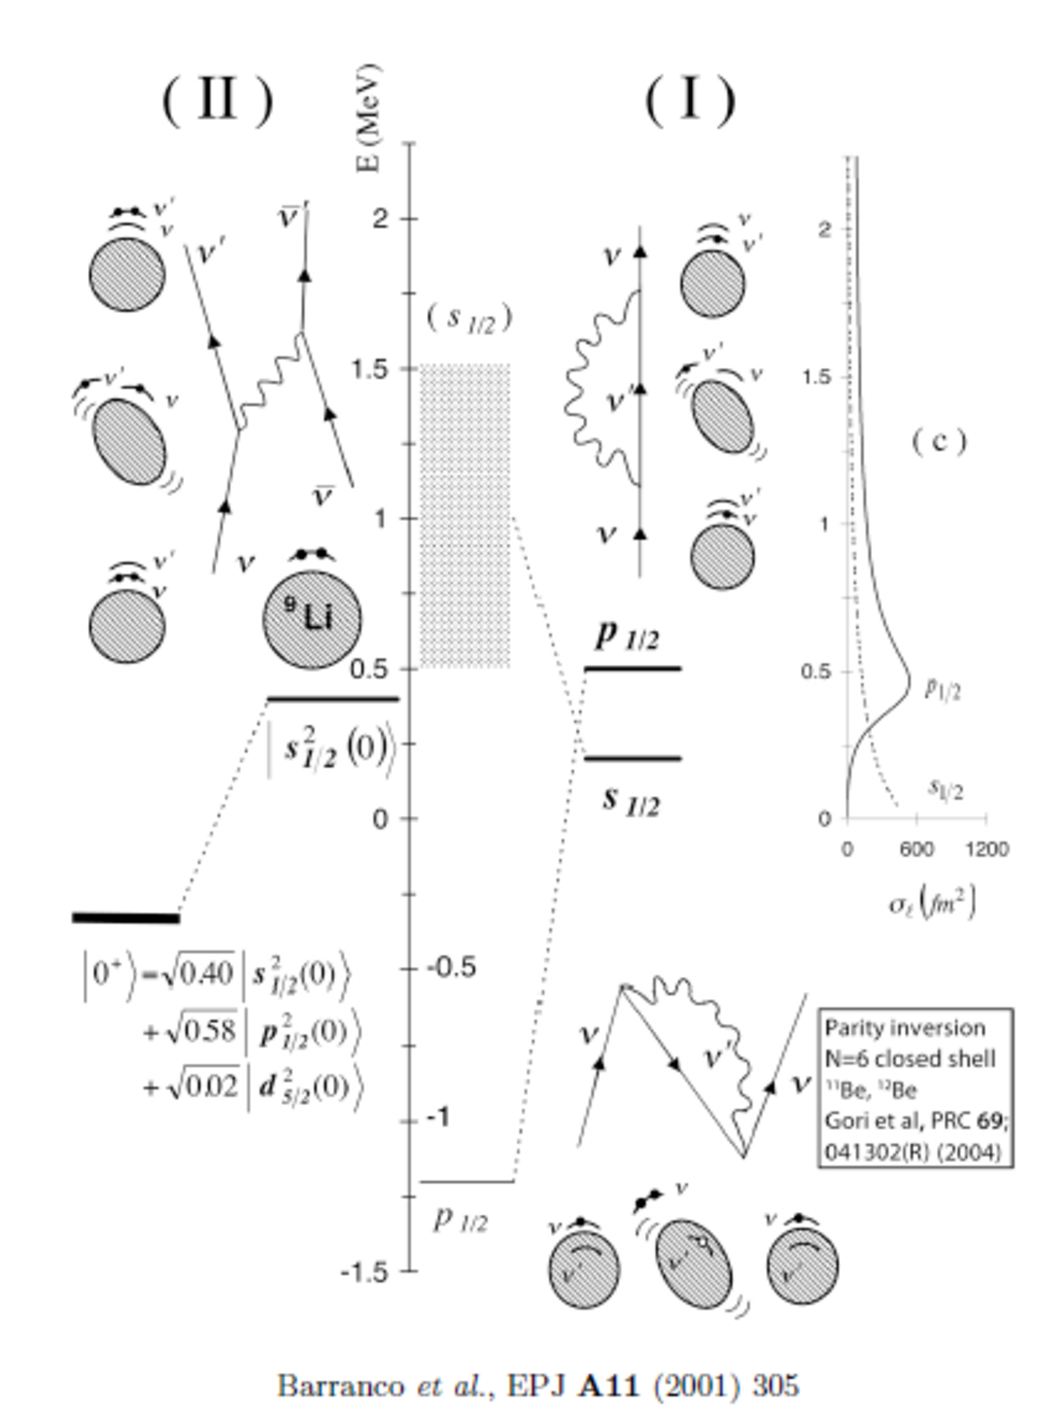
\includegraphics[width=0.7\textwidth]{figs_C4S/fig_litio}
\end{center}
\vspace{-0.5cm}
\begin{center}
 		Barranco et al., EPJ \textbf{A11} (2001) 305
\end{center}
\begin{footnotesize}
	\begin{center}
		Figure 3. Schematic representation of the dressing of single-particle and induced pairing interaction in $^{10}$Li (I), and $^{11}$Li (II), (reported with permission from Barranco et al. Eur. Phys. J. \textbf{A11} (2001) 305, Copyright 2001, European Physical Journal)
	\end{center}
\end{footnotesize}

The NFT description of the single Cooper pair system ${}^{11}$Li summarized in Fig. 3 together with the NFT reaction description of ${}^{11}$Li$(p,t) \;{}^9$Li reaction (Fig. 4), provides
\cite{Potel:10} an accurate account of the experimental findings\cite{Tanihata:08} . In particular, direct evidence for phonon mediated pairing in nuclei (see Fig. 5 of the contribution of Potel and Broglia to this Volume). At variance with the case of the infinite system (e.g. normal superconducting metals) in which there is a bound state for any strength of the interaction, in finite FMBS there is a lower limit for the strength below which the system correlates but does not condense. This is what happens around closed shell nuclei, in which the decoupling between occupied and empty states blocking pair condensation, arizes from the gap in the single--particle spectrum observed at magic numbers, and forced upon the system by the ``external'' mean field produced by all the nucleons on the motion of each single neutron and proton. As a consequence, pairing vibrations (see upper part Fig. 5) are, in atomic nuclei, strongly excited in single Cooper pair transfer reactions.

\vspace{0.3cm}

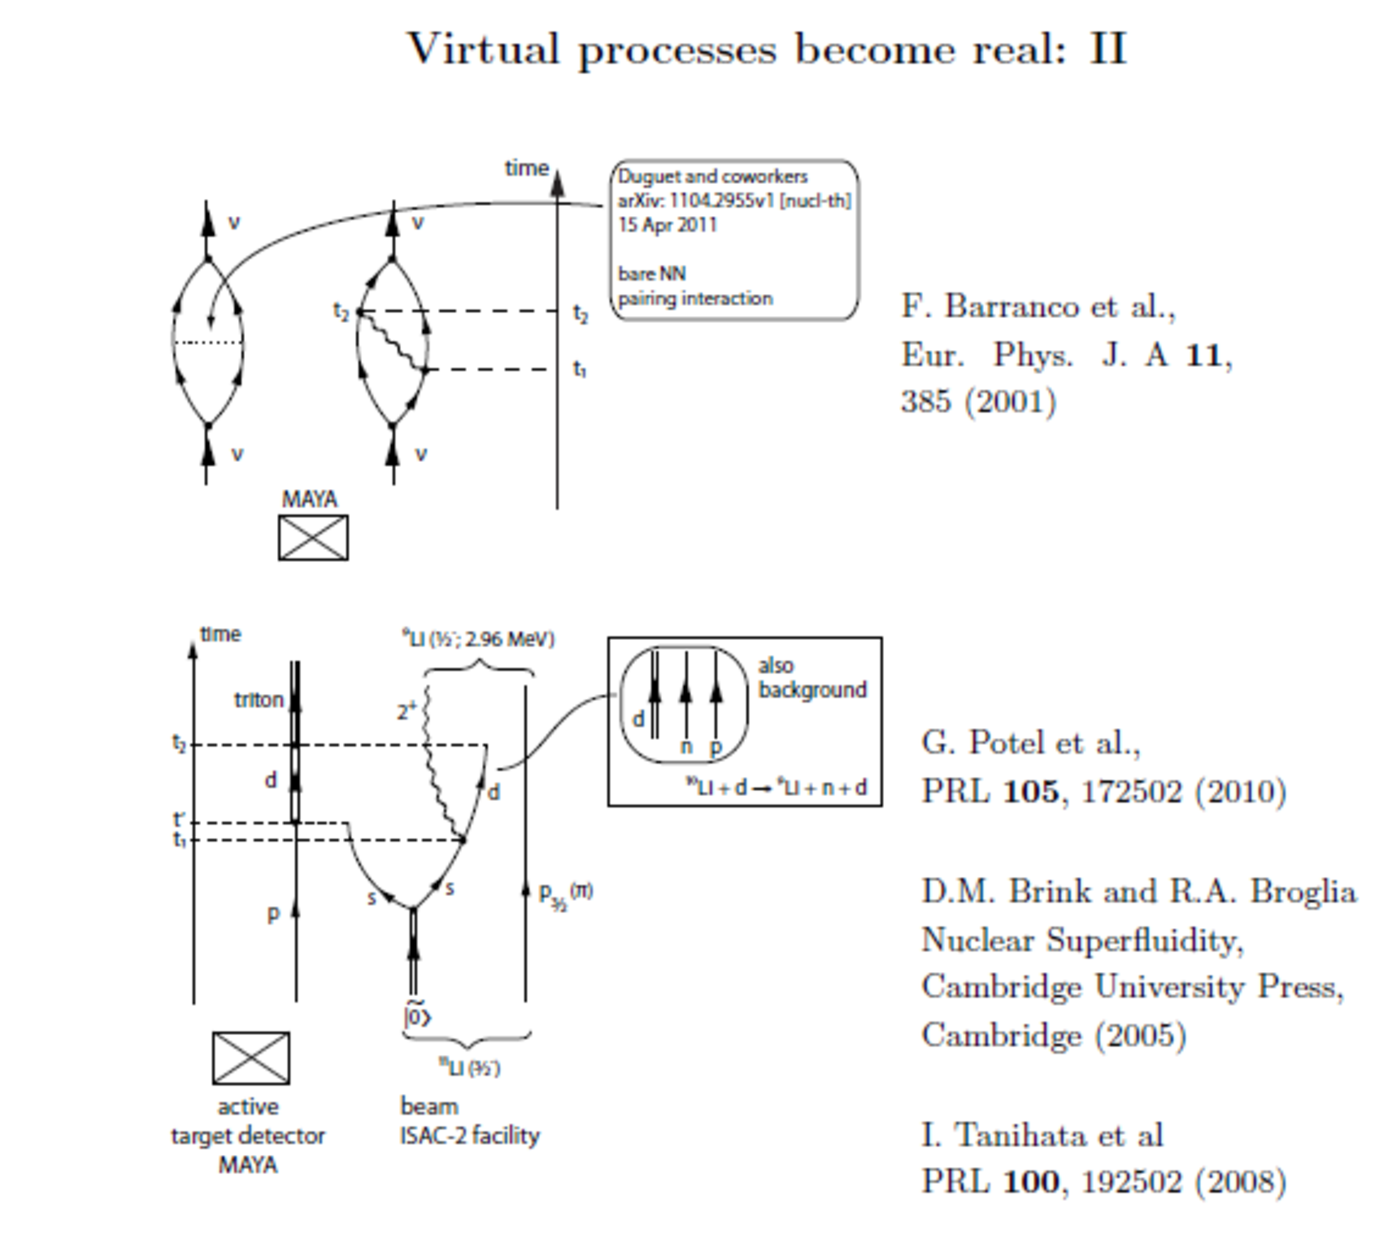
\includegraphics[width=0.8\textwidth]{figs_C4S/fig_virtual} \hspace{0.1cm} 
\begin{footnotesize}
	\begin{center}
		Figure 4. Schematic representation of the bare nucleon-nucleon and phonon induced pairing correlations (upper part) NFT diagrams, and of the excitation of the final, excited state of $^{9}$Li($1/2^{-}; 2.69$ MeV), in the TRIUMF experiment  reported in ref. \cite{Tanihata:08} (see also \cite{Potel:10}).
	\end{center}
\end{footnotesize}


%\setcounter{figure}{4}
%\begin{figure}[h!]
%	\begin{center}
%		\includegraphics[width=0.5\textwidth]{figs/fig_sym_II}
%	\caption{Schematic representation of collective modes associated with dynamical and static distortions violating rotational and gauge symmetries (see also table XI in ref. \cite{Broglia:73})}
%	\end{center}
%\end{figure}

Now, away from closed shells (open shell nuclei), such a (large) single--particle gap disappears, and one is left with rather modest differences in energy between occupied and empty states. Under such circumstances, Cooper pairs condense, the system becomes superfluid, and BCS theory provides a good description of nuclear properties. In particular the fact that the mixing between occupied and empty states gives rise to a privileged orientation in gauge space, and thus to particle number violation. The observation of pairing rotational bands (see lower part Fig. 5) being the fingerprint of nuclear spontaneous symmetry breaking in gauge space (see the Chapters of this Volume contributed by Bes, Hansen and Potel and Broglia).

\end{document}